\label{sec:results}
 
We implemented the SDP algorithm using the XADDs and tested it on several
domains. Apart from the \MarsRoverNL, we considered problems from the OR
literature such as \InventoryControl and \WaterReservoir. In the following
subsections we will study these examples empirically.
 
%%%%%%%%%%%%%%%%%%%%%%%%%%%%%%%%%%%%%%%%%%%%%%%%%%%%%%%%%%%%%%%%%%%%%%%%%%
%figure5 : time-iteration and space-iteraton for 1d-2d-noPrune inventory
\begin{figure*}[t]
\centering
%\subfigure{
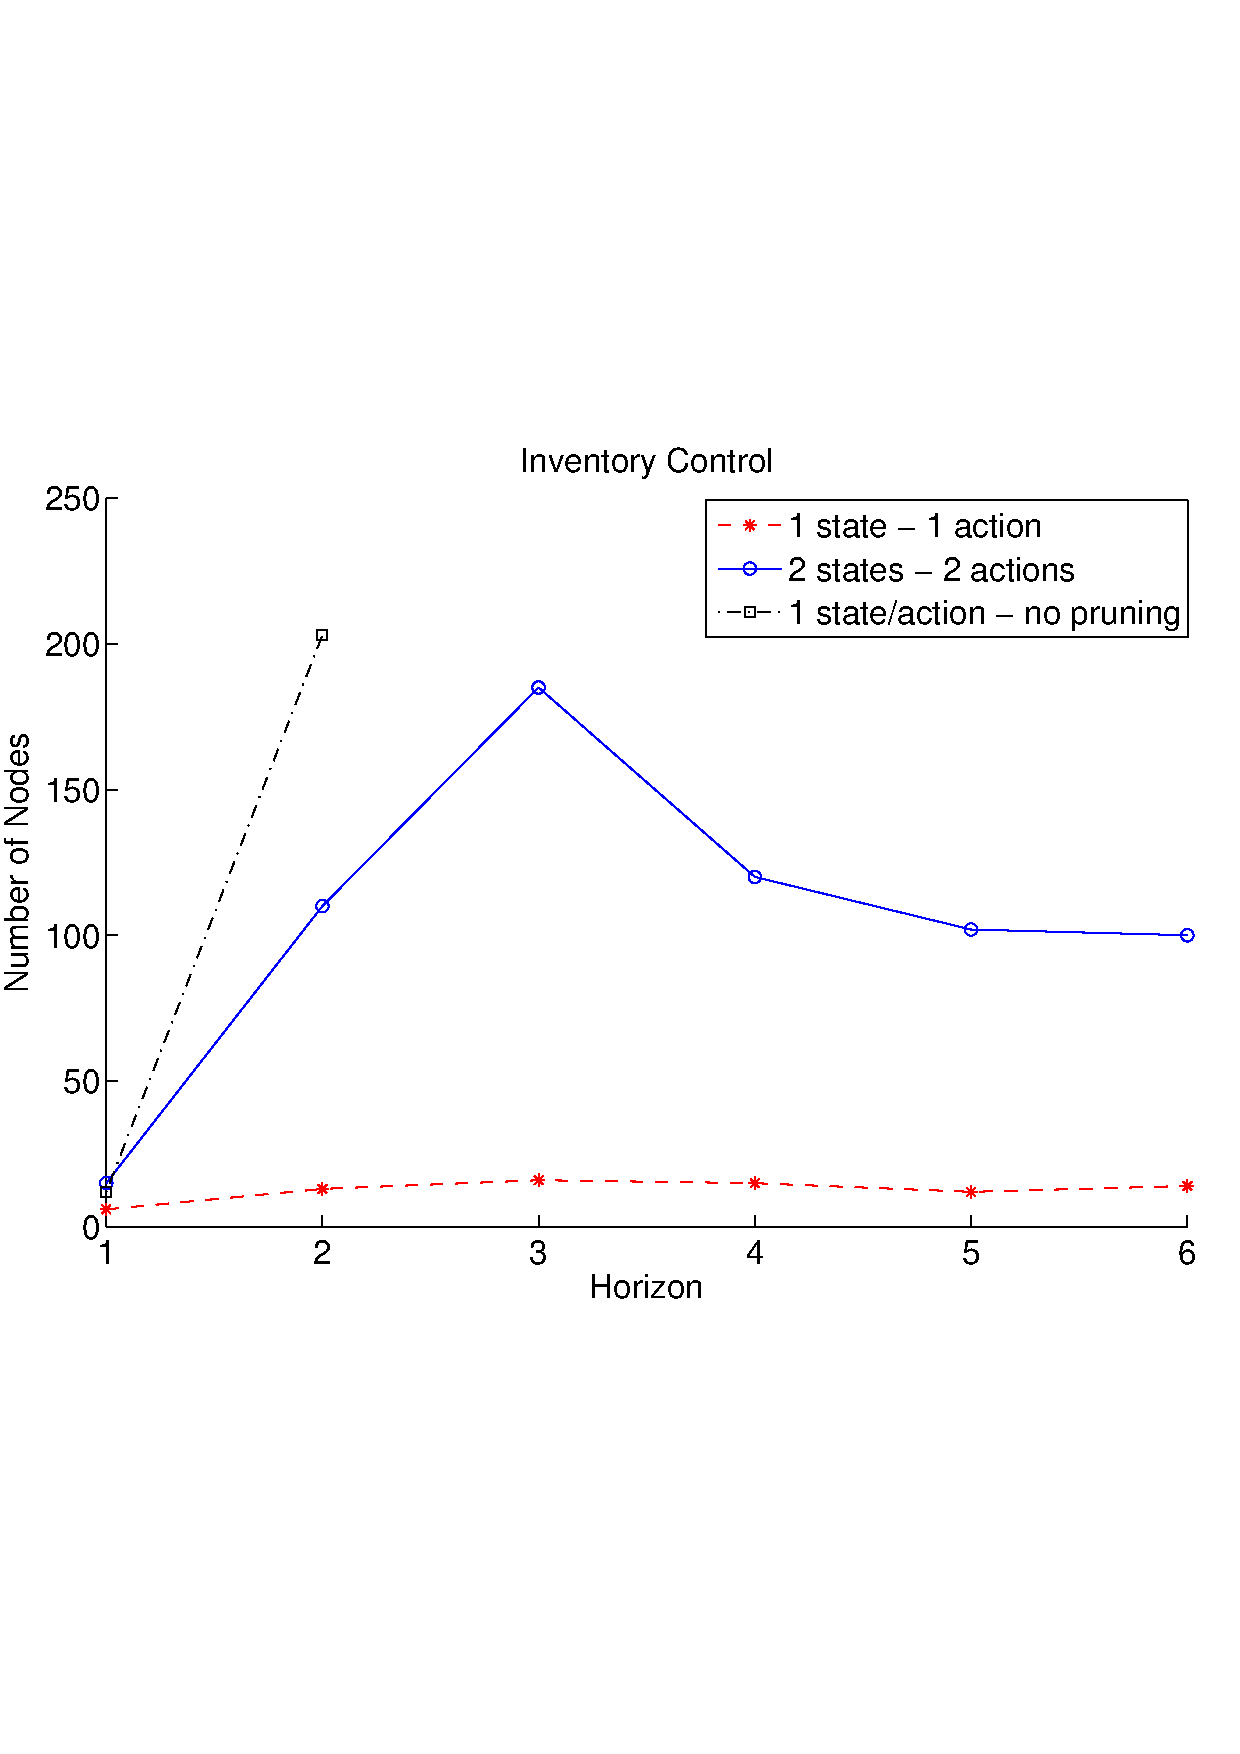
\includegraphics[width=0.47\textwidth]{Figures1/space1-3.pdf}
\hspace{5mm}
\includegraphics[width=0.47\textwidth]{Figures1/time1-3.pdf}
%}
%\vspace{-3mm}
\caption{\footnotesize
Space (\# XADD nodes in value function) and
time for different horizons of CSA-MDP on \InventoryControl\
Comparing 1D, 2D and no-pruning}
\label{fig:invC}
%\vspace{-3mm}
\end{figure*}
%%%%%%%%%%%%%%%%%%%%%%%%%%%%%%%%%%%%%%%%%%%%%%%%%%%%%%%%%%%%%%%%%%%%%%%%%%
 
\subsection{\InventoryControl}
This domain problem is a well-known optimization benchmark in the OR
literature. Business firms often deal with the problem of deciding upon the
amount of product to order in a time period so that the customer demands are
satisfied. The firm's warehouse will keep an inventory of this product to
address different customer demand levels. Each month, the firm must decide
on the amount of products to order based on the current stock level.
The order should not be too high since keeping the inventory is expensive,
nor should it be too low in which case it will be penalized for being unable
to meet customer demands and leading to the loss of customers. The
optimization problem faced by the firm is to find an optimal order policy
that maximizes the profit.~\cite{Mahootchi2009}
 
We present a simple formulation of this problem where the capacity of the
inventory is C units of each product and customer orders not satisfied in
this month are backlogged for the next month, so inventory can take negative
values. We consider two cases, a one product inventory with one order action
and the other with two products that needs two different orders.
 
We take two continuous state variable $x_1,x_2 \in [-1000,C]$ indicating the
current inventory quantity into account, with the total inventory capacity
of 800, and a stochastic boolean state variable for customer demand level
$d$ where $d=0$ is low demand levels (50) and $d=1$ is high demand levels
(150) according to some probability. \\
The continuous action variable is the order quantity $a_1,a_2 \in [0,C]$
which can at most take the value of the maximum inventory capacity. \\
 
We define an immediate negative reward for the cost of producing an order
and the storage cost of holding the products in the inventory and also a
positive reward for fulfilling the customer demand whenever there are enough
stocks in the inventory. The transition for one of the state variables and
the reward function are defined below:
%\ because of backlogging, the customer demand is always taken from the
current stock level, leaving it negative
%\ consider the next state as the current state and orders minus the
customer orders
%\ customer demands are boolean of low and high that change in every
iteration
%\
 
{\footnotesize
\begin{align*}
x'_1 & = \begin{cases}
d \wedge (x_1 + a_1 + x_2 - 150 \leq 800) : & x_1 + a_1 - 150 \\
d \wedge (x_1 + a_1 + x_2 - 150 \geq 800) : & x_1 - 150 \\
\neg d \wedge (x_1 + a_1 + x_2 - 150 \leq 800): & x_1 + a_1 - 50 \\
\neg d \wedge (x_1 + a_1 + x_2 - 150 \geq 800): & x_1 - 50 \\
\end{cases}\\
d' & = \begin{cases}
d : &(0.7)\\
\neg d: &(0.3)\\
\end{cases}\\
R & = \begin{cases}
(x_1 + x_2 \geq 900) \wedge d\\
150 - 0.5\times a_1 -0.4 \times a_2 - 0.1\times(x_1 + x_2) \\
(x_1 + x_2 \leq 900) \wedge d\\
(150 - (x_1+x_2)) - 0.5\times a_1 -0.4 \times a_2 - 0.1\times(x_1 + x_2) \\
(x_1 + x_2 \geq 300) \wedge \neg d\\
50 - 0.5\times a_1 -0.4 \times a_2 - 0.1\times(x_1 + x_2) \\
(x_1 + x_2 \leq 300) \wedge \neg d\\
(50 - (x_1+x_2)) - 0.5\times a_1 -0.4 \times a_2 - 0.1\times(x_1 + x_2) \\
\end{cases}
\end{align*}}
 
% write description in case we have to take this huge case out!
The transition for the continuous actions partitions based on the maximum
capacity of the inventory (for both products), and only adds the orders if
the current total capacity (with respect to the orders of that product and
the stocks available for both products) are less than this maximum capacity.
 
 
The demand variable is transitioned stochastically and the reward function
is based on the demand levels and the current stock in inventory. If the
current stock is larger than the total inventory, we get the reward for
fulfilling the demand $(e.g 150)$, if the demand is high and the inventory
is not high enough, then the reward is $(e.g (150 - (x_1+x_2)))$, in both
cases the action costs and holding costs are also added. This allows the
inventory to stock as many products as possible while not exceeding the
capacity of the inventory.
 
We plot the results of comparing a 1-product \InventoryControl problem with
a multi-dimensional one. Figure~\ref{fig:invC} compares the time and nodes
for different iterations for these two problem instances and a third
comparisoon for the effect of not pruning on the 1D instance. This
demonstrates the impact of having multiple constraints and action variables
on the problem size which requires much more state-action partitions. The
time and space have increased from the first iteration up to the third
iteration for the 2D problem size, but then dropped for the next horizons
due to pruning the XADD in our algorithm. As more constraints got added in
for horizon 4, they cancelled the effects of some of the previous branches
because of infeasibility and the pruning operation allows the XADD to grow
smaller in space and requiring almost a constant time depending on the
constraints added in each horizon. Without considering pruning, even the 1
product problem instance quickly falls into the curse of dimensionality
problem. In fact, after the second iteration time and space grows
exponentially and for this reason the plot fails to show the next time and
space.
% any need for 3d plot? For the 1 or 2 product case?
% any thing else we need from this example?
 
%%%%%%%%%%%%%%%%%%%%%%%%%%%%%%%%%%%%%%%%%%%%%%%%%%%%%%%%%%%%%%%%%%%%%%%%%%
%figure6 : 3d plots of refinement planning for 3 horizons
\begin{figure*}[t!]
\centering
\includegraphics[width=0.32\textwidth]{Figures1/ref1.pdf}
\includegraphics[width=0.32\textwidth]{Figures1/ref3.pdf}
\includegraphics[width=0.32\textwidth]{Figures1/ref6.pdf}
\caption{\footnotesize
Exact optimal value function for \WaterReservoir domain
}
\label{fig:reservoir}
%\vspace{-3mm}
\end{figure*}
%%%%%%%%%%%%%%%%%%%%%%%%%%%%%%%%%%%%%%%%%%%%%%%%%%%%%%%%%%%%%%%%%%%%%%%%%%
 
\subsection{\WaterReservoir}

In this experiment, we consider a continuous-time approach for the multi-reservoir domain.  
The problem of \WaterReservoir  needs to make an optimal decision on how much and when to discharge water from water reservoirs to maximize hydroelectric energy productions while considering environment constraints such as irrigation requirements and flood prevention. 

A multi-reservoir system is more desirable than the single reservoir problem due to its ability in controlling various environment parameters such as flooding.  In these systems, the inflow of downstream reservoirs are affected by the outflow of their upstream reservoirs. In the OR literature, this case  is considered much more complex and for the sake of simplicity mainly the single case in considered. For multi-reservoirs the main problem that leads to approximations to DP methods or sampling approaches is the curse of dimensionality \cite{Mahootchi2009}. Our approach handles this complexity using continuous states and actions.

The objective in this example is to find the optimal time for draining the reservoirs so that maximum reward is obtained. If draining occurs too frequently (in small time frames), flooding may occur from the excess water. This means draining should occur as latest as possible. On the other hand, not draining will cause overflow of the reservoir and waste of the energy. 

The MDP solution should solve a policy that obtains the maximum profit of electricity charges, while staying in the safe water levels of both reservoirs. In order to consider the time as a continuous variable, we allowing the system to choose to drain at any time. The choice of not draining will not gain any profit as we reward according to the electricity discharged. Two discrete actions of drain and no-drain is considered where the former is a of a continuous-time  nature. The transition function is demonstrated below: 

{\footnotesize
\begin{align*}
x_1'  = 400 * e + x1 -700 * e + 500 * e \\
x_2'  = 400 * e + x2 - 500 * e \\
\end{align*}
}
Here we take draining as the act of discharging water levels per time-step from the upper-stream reservoir to the down-stream reservoir ($500 * e$). A constant amount of discharge is always considered for the down-stream to ensure all electricity demands are fulfilled.  The amount of rain (r) is considered as a constant(400)which affects both reservoirs at the time of discharge. 

The reward function for both actions considers the safe range of [50,4500] as the safe water levels and assigns a positive reward of $e$ for the action of draining, and no rewards ( but also no penalty) for not draining. If the next state is not in the safe range, a huge penalty of -1+e6 is assigned as the reward:

{\footnotesize
\begin{align*}
(x_1\leq 4500 - 200 * e) \wedge (x2 \leq 4500 +100 *e) \\
\wedge (x_1\geq 50 - 200 * e) \wedge (x2 \geq 50 +100 *e) : e \\
\end{align*}
}
We have presented the results for this experiment next. Because of the two actions and the fact that one is continuous, we would expect to see a draining action in one iteration and a no-drain action in the next iteration, since two  draining could be performed in one longer step.

The first iteration starts with a drain only policy and achieves the value according to the current water levels of both reservoirs. The up-stream reservoir obtains the maximum value function if it has water levels above half of the safe range. The value decreases as water levels in the down-stream reservoir goes higher due to flood prevention. 

In figure \ref{fig:v2plots}, both Q-values of drain and no-drain for the second iteration have been visualized. As expected the value function follows from selecting the no-drain action. The Q-value of draining is similar to that of the first iteration and the final value function is similar to the Q-function of no-drain. The difference of the recent two value functions is in the fact that since draining was performed in the first iteration, in the second iteration, the down-stream reservoir is not in danger of flooding and can obtain the optimal value (22.5). Since flooding is a direct result of excess water in $x_1$, the optimal value is for the lower range levels in the down-stream compared to the levels of $x_2$. 
%%%%%%%%%%%%%%%%%%%%%%%%%%%%%%%%%%%%%%%%%%%%%%%%%%%%%%%%%%%%%%%%%%%%%%%%%%
% v2plot.pdf, Q-drain, Q-noDrain.pdf
% annotation?
\begin{figure*}[t]
\centering
\includegraphics[width=0.33\textwidth]{Figures1/reservoir/Q2-Drain.pdf}
\includegraphics[width=0.33\textwidth]{Figures1/reservoir/Q2-noDrain.pdf}
\includegraphics[width=0.33\textwidth]{Figures1/reservoir/v2plot.pdf}
\caption{%\footnotesize 
Value function and Q-function values of actions: Drain, No-Drain for second iteration
}
\label{fig:v2plots}
%\vspace{-3mm}
\end{figure*}
%%%%%%%%%%%%%%%%%%%%%%%%%%%%%%%%%%%%%%%%%%%%%%%%%%%%%%%%%%%%%%%%%%%%%%%%%% 

Further iterations of the exact CSA-DP algorithm results in more partitions on the state-action space. The optimal policy converges to the value obtained in the second iteration. There are some minor difference in the value of each iteration due to the fact that with higher horizons, the reservoir can plan to obtain higher rewards and prevent flooding or overflowing. We provide the Q-values of draining, not draining and the value function for iteration 9 in \ref{fig:v9plots} to show this effect. 
%%%%%%%%%%%%%%%%%%%%%%%%%%%%%%%%%%%%%%%%%%%%%%%%%%%%%%%%%%%%%%%%%%%%%%%%%%
% v9plot.pdf, Q-drain, Q-noDrain.pdf
\begin{figure*}[t]
\centering
\includegraphics[width=0.33\textwidth]{Figures1/reservoir/Q9-Drain.pdf}
\includegraphics[width=0.33\textwidth]{Figures1/reservoir/Q9-noDrain.pdf}
\includegraphics[width=0.33\textwidth]{Figures1/reservoir/v9plot.pdf}
\caption{%\footnotesize 
Value function and Q-function values of actions: Drain, No-Drain for the 9th iteration
}
\label{fig:v9plots}
%\vspace{-3mm}
\end{figure*}
%%%%%%%%%%%%%%%%%%%%%%%%%%%%%%%%%%%%%%%%%%%%%%%%%%%%%%%%%%%%%%%%%%%%%%%%%% 
Also from this plot we want to confirm the fact that in the $9^th$ iteration, the policy should choose to drain (as all other odd-iterations). The difference between the Q-values of the two actions is very minor. The sum of distances between the value function and the two Q-values shows that this distance is 49.4887 for the drain action while it is equal to 90.5312 for the no-drain action. This shows that despite the small difference, the policy tends more towards draining in this iteration. 

\section{Related Work}
The most relevant vein of Related work is that of~\cite{feng04}
and~\cite{li05} which can perform exact dynamic programming on
DC-MDPs with rectangular piecewise linear reward and transition functions
that are delta functions.  While SDP can solve these same problems,
it removes both the rectangularity and piecewise restrictions on the
reward and value functions, while
retaining exactness.  
Heuristic search approaches with formal guarantees 
like HAO*~\cite{hao09} are an attractive future extension of SDP;
in fact HAO* currently uses the method of~\cite{feng04}, which could
be directly replaced with SDP.  While~\cite{penberthy94} has considered
general piecewise functions with linear boundaries (and in fact,
we borrow our linear pruning approach from this paper), this work
only applied to fully deterministic settings, not DC-MDPs.

Other work has analyzed limited DC-MDPS having only one continuous
variable.  Clearly rectangular restrictions are meaningless with
only one continuous variable, so it is not surprising that more
progress has been made in this restricted setting.  One continuous
variable can be useful for optimal solutions to time-dependent MDPs 
(TMDPs)~\cite{boyan01}.  Or phase transitions can be used to 
arbitrarily approximate one-dimensional continuous distributions
leading to a bounded approximation approach for arbitrary single continuous
variable DC-MDPs~\cite{phase07}.  
While this work cannot handle arbitrary stochastic
noise in its continuous distribution, it does exactly solve DC-MDPs
with multiple continuous dimensions.

Finally, there are a number of general DC-MDP approximation
approaches that use approximate linear programming~\cite{kveton06}
or sampling in a reinforcement learning style approach~\cite{munos02}.
In general, while approximation methods are quite promising in
practice for DC-MDPS, the objective of this paper was to push
the boundaries of \emph{exact} solutions; however, in some sense, 
we believe that more expressive exact solutions may also inform
better approximations, e.g., by allowing the use of data structures
with non-rectangular piecewise partitions that allow higher fidelity
approximations.
